\chapter{Implementazione} %\label{1cap:spinta_laterale}
% [titolo ridotto se non ci dovesse stare] {titolo completo}
%

\begin{citazione}
In questo capitolo verrà illustrato come è stato possibile implementare la soluzione proposta e verranno illustrati anche i risultati che sono stati ottenuti
\end{citazione}

\section{Scelta del protocollo}
Al fine di procedere con il lavoro di messa in sicurezza è stato necessario scegliere uno dei protocolli \emph{Automotive} disponibili in letteratura. La prima scelta è stata \emph{FlexRay} in quanto è il protocollo più promettente e con hardware più prestante ma, sfortunatamente, dopo un'attenta ricerca in rete non è stata trovata nessuna implementazione software del protocollo. Erano disponibili solo all'acquisto delle \emph{board di testing} (con costi anche abbastanza sostanziosi) che permettevano di simulare il protocollo tramite strumentazione adeguata. Non avendo avuto fortuna con \emph{FlexRay}, la seconda scelta è ricaduta su \emph{LIN}. Purtroppo anche qui non è stato possibili trovare implementazioni \textbf{funzionanti} e \textbf{complete} del protocollo, ma solo tentativi abbandonati di implementarlo. Per queste ragioni, infine, si è scelto il protocollo \textbf{\emph{CAN}} che è supportato in maniera nativa dal kernel \textbf{Linux} tramite dei moduli appositi (oltre ad avere anche diverse implementazioni software complete e funzionanti), permettendo persino la creazione di uno o più nodi virtuali.

\section{Soluzione proposta}
Per cercare di risolvere il problema della mancanza di sicurezza all'interno del protocollo \emph{CAN}, quello che si è voluto proporre è l'\textbf{aggiunta di uno strato di cifratura} che proteggesse lo scambio di messaggi sulla rete. In particolare, si è deciso di impiegare \textbf{cifrari post-quantum} sia per garantire la massima sicurezza contro la maggior parte degli attacchi noti in letteratura sia per stabilire quale possa essere l'impatto sulle prestazioni. In seguito a questa decisione, quindi, si è deciso di impiegare per la soluzione il cifrario \textbf{AES-256} per gestire la parte di cifratura dei messaggi e \textbf{CRYSTALS-kyber-512} per far accordare i nodi della rete su una stessa chiave di sessione da utilizzare per cifrare e decifrare i messaggi.

Sostanzialmente è stato implementato un \textbf{cifrario ibrido}, ovvero un cifrario che ha una componente asimmetrica per far accordare i nodi su una stessa chiave di sessione e che ha una componente simmetrica con la quale viene utilizzata la chiave di sessione come chiave di cifratura per i messaggi che devono essere scambiati. La ragione di un cifrario del genere riguarda le \textbf{prestazioni}, poichè i cifrari asimmetrici sono estremamente più lenti dei cifrari simmetrici e, per questa ragione, non è conveniente gestire lo scambio di messaggi utilizzando solo un cifrario asimmetrico.

\section{Implementazione}
Al fine di valutare le prestazioni e la fattibilità della soluzione proprosta, è stato realizzato un applicativo molto elementare che realizza le operazioni crittografiche e utilizza \emph{CAN} per inviare dati e messaggi. Il codice contenente l'applicativo, le dipendenze e un tester può essere consultato nella repository al seguente indirizzo: \url{https://github.com/lorycris99/tesi-magistrale}.

Per l'implementazione è stato scelto di utilizzare il linguaggio \textbf{C} sia perchè le implementazioni di \emph{CAN} e delle primitive crittografiche utilizzate sono disponibili principalmente in questo linguaggio e sia per via della sua efficienza, in modo da avere una stima delle prestazioni più "realistica" possibile (solitamente anche gli applicativi reali sono scritti in \textbf{C}). Inoltre, per effettuare la compilazione dell'applicativo è necessario tener conto di alcuni accorgimenti:
\begin{itemize}
    \item Il sistema operativo su cui è stato realizzato e testato è \textbf{Ubuntu}, per cui su sistemi diversi come \textbf{Windows} non sarà possibile utilizzarlo;
    \item Dal momento che l'applicativo necessita di dipendenze che non sono presenti nei percorsi di default del \textbf{Linker}, è necessario istruirlo su dove trovare le varie librerie. Osservando il \autoref{lst:linker-info} si può vedere il comando da inviare per compilare correttamente, dove con \texttt{-L/path/to/lib} si indica la cartella dove si trovano le librerie che verranno indicate e con \texttt{-l:lib.so} si indica il nome della libreria da includere;
    \item Oltre ad istruire il \emph{Linker}, è necessario istruire anche il \textbf{Loader} poichè anche se la compilazione va a buon fine, il \emph{Loader} non troverà le librerie specificate al \emph{Linker}. Il comando da eseguire è mostrato nel \autoref{lst:loader-info} e il \textbf{path} da specificare (ovviamente) deve essere lo stesso di quello specificato al \textbf{Linker}.
\end{itemize}

\begin{lstlisting}[keywords={gcc}, caption=Istruzioni per il Linker, label=lst:linker-info]
    gcc test.c ../kyber/ref/randombytes.c -L/path/to/lib -l:libpqcrystals_kyber512_ref.so -l:libpqcrystals_aes256ctr_ref.so -l:libpqcrystals_fips202_ref.so
\end{lstlisting}

\begin{lstlisting}[keywords={export}, caption=Istruzioni per il Loader, label=lst:loader-info]
    export LD_LIBRARY_PATH=/path/to/lib
\end{lstlisting}

\begin{figure}[h]
    \centering
    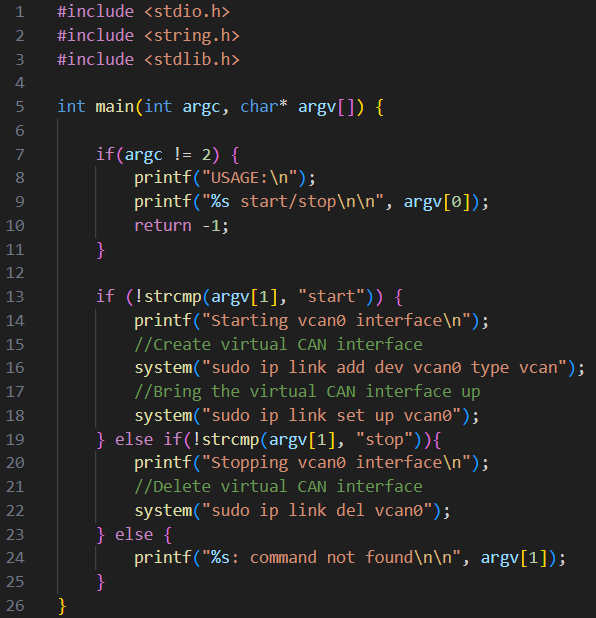
\includegraphics[width=0.6\textwidth]{capitoli/figure-implementazione/can.c.png}
    \caption{Codice sorgente del file \texttt{can.c}}
    \label{fig:can-c-code}
\end{figure}

Una volta istruiti \textbf{Linker} e \textbf{Loader} su dove trovare le librerie, quello che bisogna fare è creare un nodo \emph{CAN} con cui poter comunicare. Per essere in grado di farlo, bisogna innanzitutto abilitare il \textbf{modulo del kernel} interessato lanciando il comando \texttt{sudo modprobe vcan}, successivamente basta compilare ed eseguire il file \texttt{can.c} per avviare il nodo \emph{CAN} virtuale. Il codice del file è illustrato nella \autoref{fig:can-c-code}.


\subsection{Protocollo realizzato}
Poichè quello che si sta cercando di implementare non è presente \textbf{nativamente} in \emph{CAN}, c'è bisogno di una strategia per fare in modo da inserire all'interno del protocollo un metodo per lo scambio di chiavi e per richiedere eventualmente una nuova chiave. Essendo che \emph{CAN} lavora principalmente con gli \textbf{ID} dei messaggi, la strategia più conveniente è stata quella di utilizzare degli \textbf{ID inutilizzati dal protocollo} e assegnarli a dei messaggi \emph{personalizzati} che svolgano le operazioni aggiuntive che si vogliono implementare. Sfortunatamente, non esistono degli ID inutilizzati \textbf{universalmente} in quanto ogni casa automobilistica gestisce gli \textbf{ID} a proprio piacimento per cui bisognerebbe adattare gli \textbf{ID} caso per caso.\\
Ai fini delle simulazioni realizzate, si sono presi degli \textbf{ID bassi} (solitamente sono i meno utilizzati) e si è immaginato che non corrispondano a messaggi già assegnati. Gli \textbf{ID} utilizzati sono stati i seguenti:
\begin{itemize}
    \item $111$: messaggio che indica la presenza di una parte della \textbf{chiave pubblica} nel payload;
    \item $112$: messaggio per richiedere ad un nodo di reinviare la \textbf{chiave pubblica};
    \item $122$: messaggio che indica la presenza di una parte della \textbf{capsula} nel payload;
    \item $123$: messaggio per richiedere ad un nodo di reinviare la \textbf{capsula};
    \item $A$: messaggio che serve ad innescare la generazione di traffico casuale, utilizzato per valutare la correttezza dell'applicativo e delle operazioni di crittografia;
    \item $B$: messaggio generato casualmente e cifrato tramite \textbf{AES-256}, in risposta all'\textbf{ID} $A$;
    \item $0$: messaggio che fa terminare l'applicativo;
\end{itemize}

A questo punto, il prossimo passo è stato ideare un "protocollo" che permetta di scambiare correttamente le informazioni necessarie per concordare una chiave ma sorge anche un problema da risolvere: la lunghezza della \textbf{chiave pubblica} e della \textbf{capsula}. Un messaggio \emph{CAN} è in grado di inviare fino a 8 Byte di dati mentre una chiave pubblica di \textbf{kyber-512} è lunga 800 byte e una \emph{capsula} è lunga 768 byte, per cui la soluzione più semplice è sembrata quella di dividere entrambi in gruppi da 8 byte (avendo entrambi una lunghezza multipla di 8) e non inviare un solo messaggio ma inviarne 100 per la \textbf{chiave pubblica} e 96 per la \textbf{capsula}. A tal proposito, il protocollo ideato è il seguente:
\begin{enumerate}
    \item Invio di un messaggio contenente \textbf{ID} che specifica l'intenzione e nel payload un identificatore del nodo che lo invia;
    \item Se necessario, invio di uno o più messaggi contenenti lo stesso \textbf{ID} e nel payload il dato che si vuole inviare.
\end{enumerate}

L'invio di un identificatore come primo messaggio aiuta a distinguere chi è che ha inviato un dato, in quanto nel momento in cui viene inviata una \textbf{chiave pubblica} non è possibile capire chi l'abbia inviata (essendo una rete \emph{broadcast}) e quindi a chi associarla per inviargli, successivamente, una capsula contenente la chiave di sessione.

\subsection{Struttura del codice}
L'applicativo utilizzato per testare la soluzione è stato realizzato \textbf{ex novo} ed è stato organizzato in funzioni, ognuna delle quali assolve ad un compito specifico. Quelle principali sono:
\begin{itemize}
    \item \texttt{encrypt()}: si occupa di realizzare la cifratura di una stringa presa in input utilizzando \textbf{AES-256} in modalità \emph{CTR};
    \item \texttt{decrypt()}: si occupa di realizzare la decifratura di una stringa presa in input utilizzando \textbf{AES-256} in modalità \emph{CTR}; 
    \item \texttt{sendkey()}: si occupa di inviare la propria chiave pubblica, ottenuta con il cifrario \textbf{CRYSTALS-kyber-512}, utilizzando la rete \emph{CAN};
    \item \texttt{receivekey()}: permette di ricevere una chiave pubblica in arrivo dalla rete \emph{CAN} e la salva in un'array di chiavi "note", chiamato \texttt{publicKeys} e nella posizione corrispondente all'ID di chi ha inviato il messaggio (nel protocollo è sempre il primo messaggio);
    \item \texttt{sendCipherText()}: si occupa di inviare una capsula contenente un segreto da condividere sulla rete \emph{CAN}. La capsula viene creata nel main in seguito alla generazione di un dato casuale e, prima di inviare la capsula, viene salvato il dato in un array chiamato \texttt{sharedKeys()} e poi viene richiamata la funzione in questione passandogli la capsula;
    \item \texttt{receiveCipherTextAndSharedSecret()}: si occupa di ricevere una capsula dalla rete \emph{CAN}, la decapsula sfruttando la propria chiave privata e successivamente la salva in un array di chiavi di sessione chiamato \texttt{sharedKeys()} nella posizione corrispondente all'ID di chi ha inviato il messaggio;
    \item \texttt{cangen()}: si occupa di generare traffico casuale cifrato oppure no (in base ad un parametro). Prima che venga generato traffico, viene controllato se in corrispondenza dell'ID che ha richiesto il traffico è presente una chiave di sessione, se questa non è presente viene inviata una \textbf{richiesta di inviare un testo cifrato} (ID $123$) mentre se è presente viene inviato prima il proprio ID (per rispettare il protocollo), poi viene inviato il numero di messaggi che saranno mandati (per aiutare l'interlocutore a sincronizzarsi) e successivamente vengono inviati i messaggi cifrati con la chiave di sessione;
    \item \texttt{receiveCangen()}: si occupa di ricevere il traffico generato sulla rete \emph{CAN} e decifrarlo se necessario;
    \item \texttt{intToHex()}: funzione ausiliaria che si occupa di convertire un numero \textbf{intero} in un numero \textbf{esadecimale};
    \item \texttt{hexToInt()}: funzione ausiliaria che si occupa di realizzare l'inverso di \texttt{intToHex()}
    \item \texttt{main()}: funzione principale che realizza l'applicativo e si occupa di generare la coppia di chiavi pubblica e privata e di richiamare le funzioni corrette alla ricezione di un determinato ID \emph{CAN}. Si occupa anche di effettuare controlli (come quello precedente alla chiamata di \texttt{cangen()}) e operazioni ausiliarie.
\end{itemize}

\section{Librerie utilizzate}
Per realizzare tutte le funzionalità dell'applicativo con relativa cifratura e comunicazione tramite protocollo \emph{CAN}, è stato necessario utilizzare delle librerie esterne (sempre in linguaggio \textbf{C}) che implementassero le operazioni richieste. Le librerie utilizzate sono:
\begin{itemize}
    \item CAN-utils;
    \item Kyber;
    \item OpenSSL.
\end{itemize} 

\subsection{CAN-utils}
Il cuore dell'intero progetto, è la libreria (come si intuisce dal nome) che realizza le primitive di comunicazione tramite protocollo \emph{CAN}. Inoltre, questa lavora in sinergia con il \textbf{sottosistema \emph{CAN} per Linux} (chiamato \textbf{SocketCAN}) offrendo moltissimi strumenti per interfacciarsi con tale modulo. Affinchè si possa utilizzare correttamente, bisogna creare un'interfaccia \emph{CAN} virtuale (utilizzando il file \texttt{can.c} come visto in \autoref{fig:can-c-code}) e successivamente utilizzare le funzioni specificando il nome dell'interfaccia (all'interno del progetto è stato utilizzato il nome \texttt{vcan0}). Nonostante sia completo di molte funzioni, all'interno del progetto è stata utilizzata solo una piccola parte di queste:

\begin{itemize}
    \item \texttt{cangen}: funzione che permette di generare del traffico in maniera totalmente casuale o casuale ma in base a dei parametri (ID fissato, lunghezza del payload fissata, ecc.);
    \item \texttt{candump}: funzione che permette di leggere il traffico inviato ad un'interfaccia \emph{CAN} virtuale, visualizzando in maniera semplice l'ID, la lunghezza del payload e il payload;
    \item \texttt{cansend}: funzione che permette di inviare un singolo messaggio \emph{CAN} specificando tutti i parametri compreso il payload.
\end{itemize}

\subsection{Kyber}
Per aggiungere al progetto il cifrario \textbf{Kyber-512}, è stata utilizzata la libreria ufficiale realizzata dal gruppo \textbf{pq-crystals}, autori del cifrario in questione e di altri (sempre \textbf{Post-Quantum}). Questa offre tutte le funzionalità del \emph{KEM} \textbf{kyber} rendendo disponibile anche una versione dell'implementazione ottimizzata per i processori realizzati da \textbf{Intel} (quindi con architettura chiamata \textbf{x86}) ma, tuttavia, è stata utilizzata l'implementazione di riferimento e non quella ottimizzata, poichè una \emph{ECU} potrebbe utilizzare un processore con architettura differente e quindi i risultati potrebbero non essere realistici. Per poterla utilizzare all'interno del progetto, è stato necessario creare delle \textbf{librerie condivise} (seguendo la guida fornita con l'implementazione) che, spiegato in maniera molto semplice, sono dei file compilati in maniera tale da poter essere utilizzati in altri progetti in maniera del tutto indipendente.\\
Tra le funzioni offerte, quelle utilizzate sono:
\begin{itemize}
    \item \texttt{pqcrystals\_kyber512\_ref\_keypair()}: funzione che permette di creare una coppia di chiavi, una pubblica e una privata, in modo da poter utilizzare il cifrario (\autoref{fig:kyber-keypair});
    \item \texttt{pqcrystals\_kyber512\_ref\_enc()}: funzione che genera un dato casuale chiamato \emph{shared secret} e lo \textbf{incapsula} all'interno di una capsula chiamata \emph{ciphertext} utilizzando una \textbf{chiave pubblica} fornita in input (\autoref{fig:kyber-enc});
    \item \texttt{pqcrystals\_kyber512\_ref\_dec()}: funzione che \textbf{decapsula} lo \emph{shared secret} dalla capsula utilizzando la \textbf{chiave privata} correlata alla chiave pubblica utilizzata per creare la capsula (\autoref{fig:kyber-dec}).
\end{itemize}

\begin{figure}[h]
    \begin{subfigure}{0.45\textwidth}
        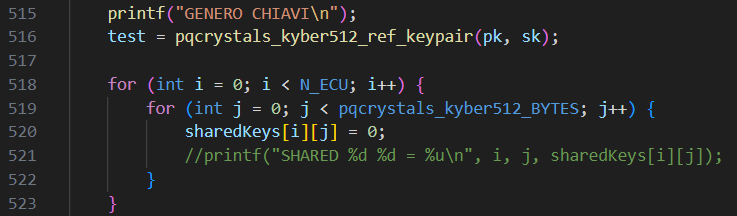
\includegraphics[width=1\textwidth]{capitoli/figure-implementazione/kyber-keypair.png}
        \caption{Utilizzo della funzione \texttt{keypair}}
        \label{fig:kyber-keypair}
    \end{subfigure}
    \begin{subfigure}{0.45\textwidth}
        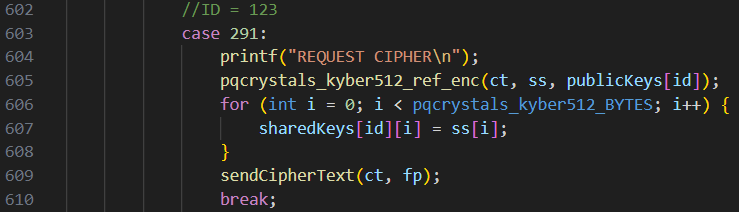
\includegraphics[width=1\textwidth]{capitoli/figure-implementazione/kyber-enc.png}
        \caption{Utilizzo della funzione \texttt{enc}}
        \label{fig:kyber-enc}
    \end{subfigure}
    \centering
    \begin{subfigure}{0.5\textwidth}
        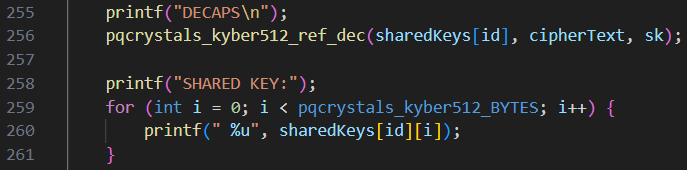
\includegraphics[width=1\textwidth]{capitoli/figure-implementazione/kyber-dec.png}
        \caption{Utilizzo della funzione \texttt{dec}}
        \label{fig:kyber-dec}
    \end{subfigure}
    \caption{Utilizzo delle funzioni di \textbf{Kyber}}
    \label{fig:kyber-functions}
\end{figure}

Sebbene le funzionalità offerte siano complete e funzionanti, questa libreria ha una mancanza che non permette di sfruttare le piene potenzialità di \textbf{kyber}, ovvero si limita ad implementare solo la funzionalità \emph{KEM} e quindi facendolo lavorare solo con dati casuali e non scelti. È una limitazione importante poichè \textbf{kyber}, analogamente a \textbf{RSA}, può essere usato anche come \textbf{cifrario a chiave pubblica} (cifrando messaggi arbitrari \textbf{scelti}) e non solo come \emph{KEM} per lo scambio di \textbf{chiavi di sessione} (quindi con messaggi casuali generati \textbf{ad-hoc}). Tuttavia, all'interno del progetto questa limitazione non ha avuto nessun impatto sull'applicativo realizzato, ma ha semplicemente reso la fase di testing della correttezza dei messaggi leggermente più complicata.

\subsection{OpenSSL}
Per includere nel progetto il cifrario \textbf{AES} è stata utilizzata una libreria della \emph{suite} \textbf{OpenSSL}, una raccolta di strumenti crittografici completa, efficiente e inclusa nativamente all'interno del kernel \textbf{Linux}. Molto potente e utilizzabile nativamente su sistemi operativi basati su \textbf{Linux}, questa raccolta offre moltissimi cifrari oltre \textbf{AES} e, in merito a quest'ultimo, fornisce anche l'implementazione di tutte le sue modalità operative. Infatti, nel progetto è stata utilizzato \textbf{AES-256} in modalità \textbf{CTR}, in quanto nella libreria di \textbf{kyber} viene fatto riferimento a questa e, per evitare eventuali problemi di compatibilità, è stata usata tale modalità.\\
Per poter essere in grado di sfruttare la libreria basta semplicemente includere le librerie di OpenSSL \texttt{evp.h}, \texttt{conf.h} e \texttt{err.h}, successivamente realizzare una o più funzioni che richiamino le operazioni di cifratura e decifratura. All'interno del progetto sono state realizzate due fuzioni:
\begin{itemize}
    \item \texttt{encrypt()}: funzione che si occupa di preparare \textbf{AES} per la cifratura leggendo i parametri forniti (chiave di cifratura, nonce e lunghezza del testo da cifrare) e di effettuare la cifratura del \textbf{testo in chiaro}, come mostrato in \autoref{fig:aes-encrypt}.
    \item \texttt{decrypt()}: funzione che si occupa di preparare \textbf{AES} per la decifratura leggendo i parametri forniti (come per la cifratura) e di effettuare la decifratura del \textbf{testo cifrato}, come mostrato in \autoref{fig:aes-decrypt}.
\end{itemize}

\begin{figure}[h]
    \begin{subfigure}{0.45\textwidth}
        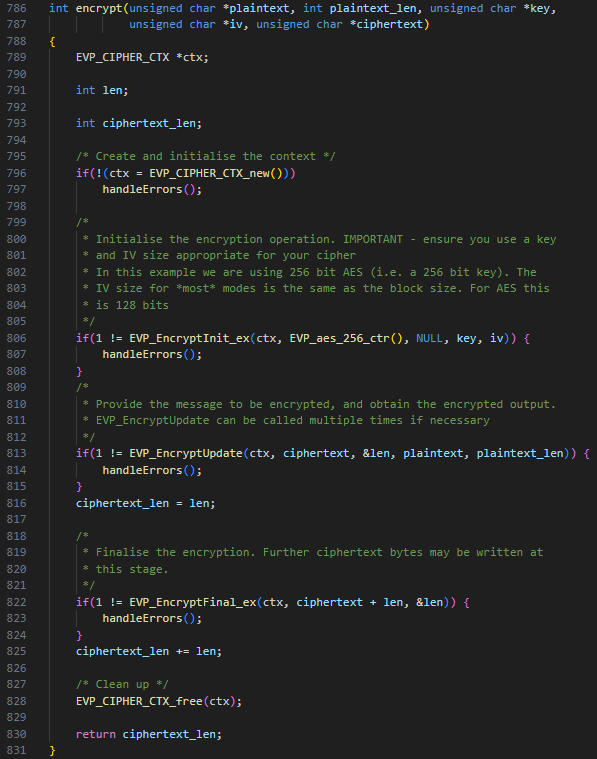
\includegraphics[width=1\textwidth]{capitoli/figure-implementazione/aes-encrypt.png}
        \caption{Funzione per l'operazione di \textbf{cifratura}}
        \label{fig:aes-encrypt}
    \end{subfigure}
    \begin{subfigure}{0.45\textwidth}
        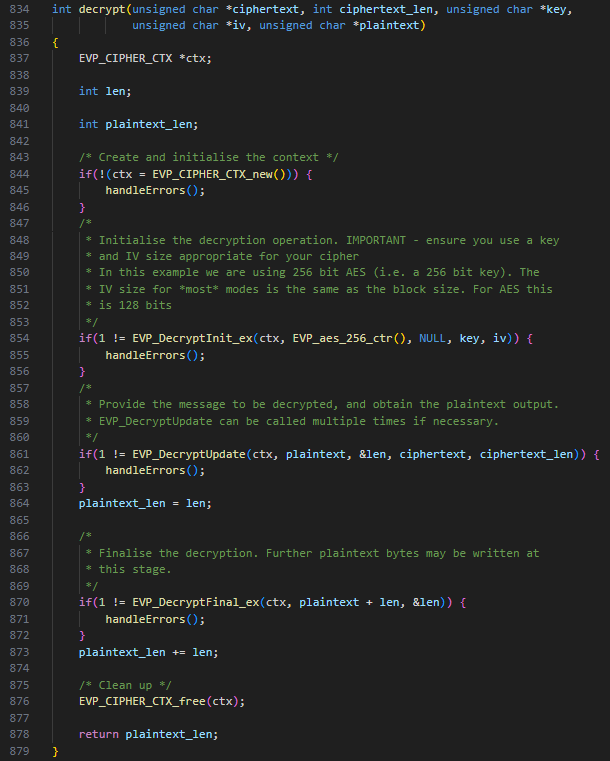
\includegraphics[width=1\textwidth]{capitoli/figure-implementazione/aes-decrypt.png}
        \caption{Funzione per l'operazione di \textbf{decifratura}}
        \label{fig:aes-decrypt}
    \end{subfigure}
    \caption{Implementazione del cifrario \textbf{AES-256-CTR}}
    \label{fig:aes-functions}
\end{figure}

\section{Difficoltà riscontrate}
Durante la realizzazione dell'applicazione sono state riscontrate diverse difficoltà, principalmente riguardo l'utilizzo delle librerie.
\subsection{Introduzione di CAN-utils}
La difficoltà più complicata da gestire è stata l'introduzione della libreria \textbf{CAN-utils}, in quanto questa è stata rilasciata come strumento \emph{indipendente} e non è stata prevista la possibilità di utilizzarlo come \textbf{libreria}. Per questo motivo è stato necessario adottare una strategia per utilizzare gli eseguibili di \textbf{CAN-utils} (ottenuti effettando la compilazione dei \emph{codici sorgenti}) all'interno dell'applicativo realizzato. La strada seguita, quindi, è stata quella di richiamare gli eseguibili tramite linea di comando, utilizzando la funzione \emph{system()} offerta dalla libreria \texttt{stdlib.h} offerta da \textbf{C}, la quale non fa altro che creare un nuovo processo ed eseguire il comando \texttt{sh -c STRINGA\_INPUT}. In questo modo, se si costruisce una \textbf{stringa} che corrisponde al comando completo da eseguire (compreso di argomenti e parametri) e si esegue la funzione con questa stringa, quello che si ottiene è che viene eseguita l'operazione, ovviamente a patto che la stringa non contenga errori. Un esempio, estratto dal codice, può essere visto nel \autoref{lst:canutils-adapt}.

\begin{lstlisting}[language=C, caption=Utilizzo di CAN-utils tramite linea di comando, label=lst:canutils-adapt]
    // Invio ID e numero di messaggi
    char* idToSend = "../can-utils-2023.03/cansend vcan0 00B#";
    int sendLen = strlen(idToSend);
    char* preCmd = malloc( (sendLen + 20) * sizeof(char));
    strcpy(preCmd, idToSend);
    strcat(preCmd, ID_ECU);
    system(preCmd);
\end{lstlisting}

\subsection{Utilizzo delle \emph{pipe}}
Purtroppo il semplice utilizzo della funzione \texttt{system()} non è bastata per utilizzare la libreria. Questo perchè la funzione si limita semplicemente all'esecuzione del codice che gli viene fornito, senza restituire un'eventuale \textbf{output} generato dall'esecuzione del comando. Ad esempio se si esegue \texttt{candump} per leggere i messaggi che viaggiano sulla rete con \texttt{system()}, quello che succede è che oltre a non mostrare nessun output, il codice si blocca in quanto \texttt{candump} è \textbf{bloccante} (poichè rimane in ascolto perpetuo di messaggi). Per risolvere questo problema, bisogna utilizzare un altro strumento: le \textbf{pipe}.

Una \textbf{pipe} è uno strumento di \textbf{comunicazione tra processi} che consiste nella creazione di un canale unidirezionale tra un processo e un altro, ovvero solo uno di due processi può \textbf{scrivere} sulla \emph{pipe} e solo l'altro può \textbf{leggere} dalla \emph{pipe}. Alcuni vantaggi dell'utilizzo di una \emph{pipe} sono:
\begin{itemize}
    \item Semplicità: sono un modo semplice e diretto per far cominicare due processi;
    \item Efficienza: permettono di trasferire dati velocemente e con il minimo \emph{overhead};
    \item Affidabilità: sono in grado di effettuare la rilevazione di errori durante la trasmissione e di assicurare la corretta consegna dei dati;
    \item Flessibilità: permettono di realizzare tantissimi tipi di protocollo di comunicazione, sia unidirezionali che bidirezionali (aprendo due pipe in versi opposti). \cite{geeksforgeeks_pipe}
\end{itemize}

Tuttavia, l'utilizzo di una \emph{pipe} presenta anche alcuni svantaggi:
\begin{itemize}
    \item Capacità limitata: non hanno una capienza adeguata per eventuali enormi quantità di dati trasferite in una sola volta, limitandosi solo con piccole quantità di dati;
    \item Unidirezionale: come già accennato, permettono una comunicazione solo in un verso e, se si desidera realizzare una comunicazione bidirezionale, bisogna necessariamente creare una seconda \emph{pipe} nel verso opposto alla prima;
    \item Sincronizzazione: nel caso di una comunicazione bidirezionale, è necessario che entrambi i processi siano sincronizzati per assicurare che la trasmissione avvenga nell'ordine corretto; 
    \item Scalabilità limitata: sono limitate ad una comunicazione tra pochi processi su uno stesso computer. \cite{geeksforgeeks_pipe}
\end{itemize}

Utilizzando una \emph{pipe}, quindi è possibile ottenere l'output di un processo in esecuzione e, sfruttando questa caratteristica, è possibile intercettare i messaggi letti con \texttt{candump}. Come si può vedere nel \autoref{lst:pipe-creation}, utilizzando la funzione \texttt{popen()} si crea una \emph{pipe} con un nuovo processo che eseguirà il comando fornito in input come stringa (stessa logica di \texttt{system()}) e si può specificare se il processo che ha lanciato \texttt{popen()} leggerà dalla \emph{pipe} (con il parametro "r") o scriverà sulla \emph{pipe} (con il parametro "w").

\begin{lstlisting}[language=C, caption=Creazione di una pipe, label=lst:pipe-creation]
    // Mi metto in ascolto sul bus
    FILE* fp = popen("../can-utils-2023.03/candump vcan0", "r");
\end{lstlisting}

Per poter leggere dalla pipe si può utilizzare una qualsiasi funzione che legge da uno \textbf{stream}, nel caso del progetto è stata utilizzata la funzione \texttt{fgets} come mostrato nel \autoref{lst:pipe-read}.

\begin{lstlisting}[language=C, caption=Lettura dalla pipe, label=lst:pipe-read]
    fgets(buffer, 50, fp);
    j = 9;
        k = 0;
        // Ottengo l'ID che definisce la tipologia di messaggio
        while (!isspace(buffer[j])) {
            msgCode[k] = buffer[j];
            k++;
            j++;
            
        }
        j = 0;
        // Estraggo l'ID del sender
        for(int i = 0; i < DATA_LENGTH; i+=2) {
            tempID[i] = buffer[20 + j];
            tempID[i+1] = buffer[20 + j +1];
            j+=3;
        }
        tempID[DATA_LENGTH] = '\0';
\end{lstlisting}
Ovviamente, quello che si legge dalla pipe è una stringa, quindi è necessario effettuare un \emph{post-processing} di questa per estrarre le informazioni contenute. Un esempio di \emph{post-processing} si trova sempre nel \autoref{lst:pipe-read}.

\subsection{Chiusura della pipe}
Al termine di ogni programma, è buona norma liberare tutto lo spazio allocato, chiudere tutti i file aperti, chiudere tutte le pipe create, ecc. al fine di evitare possibili problemi di \textbf{memory leak} o inconsistenze. Quindi, al fine di seguire queste \emph{best-practices}, come ultime operazioni da eseguire prima del termine dell'applicativo si cerca di chiudere la \emph{pipe} creata ma, tuttavia, quello che succede è che il programma si ferma e non prosegue (quindi non termina). Questo problema è dovuto al fatto che quando si chiude una pipe, la funzione \texttt{pclose()} (necessaria per chiudere una \emph{pipe}) \textbf{attende che il processo collegato alla \emph{pipe} termini} \cite{linux_man_page_pipe}, evento che non accadrà mai poichè (come accennato in precedenza) \texttt{candump} si mette in ascolto \textbf{perpetuo}. Quindi, per chiudere la \emph{pipe} è necessario \textbf{terminare forzatamente} il processo creato da \texttt{popen} ma, anche qui, sorge un ulteriore problema, ovvero non si conosce nessuna informazione riguardo il processo creato. Per poter chiudere un processo è necessario sapere il suo ID (chiamato \textbf{PID}) e inviare un segnale di interruzione, ma le uniche informazioni note (anche grazie alla documentazione di \texttt{popen}) sono che il processo è \textbf{figlio} di quello che chiama la funzione \texttt{popen} e che il nome del processo è esattamente il comando lanciato per eseguirlo, quindi è necessario adottare una strategia per ottenere il \textbf{PID} del processo figlio. Dopo un'attenta ricerca e vari tentativi, la strategia vincente è stata la seguente:
\begin{enumerate}
    \item Ottenimento del \textbf{PID} del processo padre tramite la funzione \texttt{getpid()};
    \item Utilizzo del comando \texttt{ps -eaf} tramite la costruzione di una stringa assemblata con il \textbf{PID} del padre e il nome del processo;
    \item Creazione di una \emph{pipe} sul comando appena costruito in modo da ottenere l'output di quest'ultimo;
    \item Lettura dalla \emph{pipe} ed estrazione del \textbf{PID} del processo figlio;
    \item Invio del segnale di terminazione al processo figlio;
    \item Chiusura di entrambe le \emph{pipe}.
\end{enumerate}

Il codice necessario per implementare questa strategia si può trovare nel \autoref{lst:pipe-close}, con l'aggiunta di ulteriori commenti per rendere più chiaro ogni punto.

\begin{lstlisting}[language=c, caption=Operazioni necessarie per chiudere la \emph{pipe}, label=lst:pipe-close]
    // Termino il processo associato alla pipe
    pid_t pid = getpid();
    char num[8];
    sprintf(num, "%d", pid);

    // Comando da lanciare per ottenere il PID del processo figlio
    char* cmd = "ps -eaf | grep \"../can-utils-2023.03/candump vcan0\" | grep ";
    int tempLen = strlen(cmd) + 8;
    char* temp = malloc(tempLen * sizeof(char));
    strcpy(temp, cmd);
    // Aggiungo il PID del processo padre al termine della stringa
    strcat(temp, num);
    
    // Creo una nuova pipe sul comando per ottenere l'output di questo
    FILE* targetProcess = popen(temp, "r");

    // Leggo dalla nuova pipe
    fgets(buffer, 50 ,targetProcess);

    // Estraggo il PID dalla stringa ottenuta
    int i = 0;
    while(!isspace(buffer[11 + i])) {
        num[i] = buffer[11 + i];
        i++;
    }

    int targetPid;
    sscanf(num, "%d", &targetPid);

    // Termino il processo figlio
    kill(targetPid, SIGKILL);

    free(temp);

    // Chiudo sia la pipe di supporto che la pipe principale
    pclose(targetProcess);
    pclose(fp);
    printf("CHIUSA LA PIPE\n");
\end{lstlisting}

\section{Risultati ottenuti}
Una volta completato l'applicativo e risolti tutti i problemi riscontrati, il passo successivo è stato quello di misurare l'\textbf{impatto prestazionale} apportato dall'aggiunta della cifratura. Sono stati raccolti due tempi, il tempo necessario per generare le chiavi di cifratura e il tempo necessario per lo scambio dei messaggi, entrambi in \textbf{microsecondi}.

\subsection{Tempi per la generazione delle chiavi}
Il tempo medio necessario per la generazione delle chiavi e per lo scambio di una chiave di sessione tra due nodi è di circa $50829\ \micro s$. A livello prestazionale, assumento che avvenga all'avvio della rete, l'impatto prestazionale non è elevato ma è comunque \textbf{molto alto}, in quanto è necessario scambiare una grande quantità di messaggi per inviare capsula e chiave pubblica (quasi 200 per ogni nodo). Per cui potrebbero essere introdotti dei ritardi che, su reti contenenti molte \emph{ECU} potrebbero essere percettibili dall'uomo e allungare i tempi di accensione di tutti i sistemi.

\subsection{Tempi per lo scambio di messaggi}
Per quanto riguarda il tempo necessario per lo scambio di messaggi, un confronto può essere visto in \autoref{table:times}. I tempi sono stati raccolti a partire dall'inizio della cifratura e fino alla decifratura dell'ultimo byte (in pratica quando il contenuto del messaggio è disponibile all'applicativo), quindi considerando anche eventuali ritardi in trasmissione. A differenza del precedente, questo impatto è \textbf{molto elevato}, in quanto si introduce un ritardo per trasmissione di quasi $100\ ms$, inaccettabile per sistemi \emph{safety-critical} e per la gestione di un motore di un'auto in corsa.

\begin{table}[h]
    \centering
    \begin{tabular}{| c | c |}
        \hline
        \large{\textbf{Tempo medio senza cifratura}} & \large{\textbf{Tempo medio con cifratura}} \\
        \hline
        $93.12\ \micro s$ & $96433.16\ \micro s$ \\
        \hline
    \end{tabular}
    \caption{Tempi medi rilevati}
    \label{table:times}
\end{table}

Se si considera un'auto in corsa ad una velocità di $180\ km/h$, un ritardo di trasmissione di circa $100\ ms$ corrispondono a circa $5\ m$ percorsi senza nessuna risposta dai comandi e senza considerare un eventuale ritardo aggiuntivo necessario per processare il messaggio. Prendendo per esempio un sistema \textbf{brake-by-wire}, $5\ m$ di frenata in più possono fare una grande differenza ed evitare incidenti (anche mortali).
\newpage
